
\graphicspath{{./chap4/images/}}  
\chapter{Environments}

\textbf{이 장은 기본 연구 환경을 다룬다.}
\section{주의사항}
\begin{itemize}
 \item \textbf{sudo reboot은 그 어떠한 경우에도 사용하면 안 된다.} 새로운 프로그램을 설치하는 등 작업 도중 블로그 글을 따라쓰게 될 수 있는데, 그중에 reboot 명령어가 있으면 건너뛰자. 타인의 프로세스가 비정상적으로 종료될 위험이 크다.
 \item \textbf{모든 사용자는 반드시 가상환경을 구성하고, 그 가상환경 내에 여러가지 연구에 필요한 프로그램들을 설치해 사용해야 한다.} 이렇게 하면 관리자 권한 없이 원하는 대로 프로그램의 버전이나 설정을 바꿀 수 있다.
\end{itemize}


	 
아래는 설치 방법들을 설명할 것인데, 어렵다면 그냥 마지막 부분만 확인해도 된다.
\section{쉘 바꾸기(선택)}
 쉘이 뭔지에 대한 장황한 설명을 쓰지는 않겠다. 쉘에는 sh, bash 등이 있는데, 처음 아이디를 만들면 쉘이 sh로 설정이 되어있을 수 있다. bash가 여러가지 좋은 기능(위 아래 방향키로 이전 명령 불러오기 등)이 있으므로 다음 명령어를 쳐서 bash로 쉘을 바꿔주자.
\begin{lstlisting}
    $ chsh -s /bin/bash
\end{lstlisting}
이후 서버와의 연걸을 한 번 끊었다가 재접속했을 때 아래처럼 \$ 옆에 사용자명이 뜨면 성공한 것이다.
\begin{figure}[H]
	\begin{center}
        
\includegraphics[width=5cm]{bash}
        \caption{bash로 변경}
    \end{center}
\end{figure}
현재 서버에서 bash 쉘을 사용하는 상태에서 GPU를 사용하는 프로그램을 실행시키는 경우, GPU에 메모리만 할당되고 GPU를 사용하지 않는 현상이 종종 나타나고 있으니 만약 bash 쉘을 사용하는데 GPU 사용량이 이상할 만큼 저조하다면, 이를 한 번 의심해보자. 해당 프로그램을 실행시킬 때에만 bash를 사용하지 않으면 이러한 문제를 해결할 수 있다.
\section{가상환경 설치}
다음 명령어로 가상환경을 설치하자. 
\begin{lstlisting}
    $ virtualenv venv
    $ virtualenv venv --python=python3.6
\end{lstlisting}
여기서 3.5 대신 원하는 다른 버전을 다운받아도 된다. \\
만약 다음과 같은 메세지와 함께 
이후 가상환경을 사용할 때에는 다음 명령어를 사용하면 된다.
\begin{lstlisting}[language=bash]
    $ source ~/venv/bin/activate
\end{lstlisting}
\begin{figure}[H]
	\begin{center}
        
\includegraphics[width=0.6\linewidth]{venv}
        \caption{활성화된 venv 환경}
    \end{center}
    \end{figure}
\section{tensorflow 설치}
가상환경을 켠 상태로 다음 명령어를 입력하자.
\begin{lstlisting}
    $ pip3 install --upgrade tensorflow
\end{lstlisting}
\section{CUDA 설치}
만약 서버에 없는 \acs{CUDA}가 필요하다면 관리자에게 문의해야 한다. 이후 자신의 환경변수에 설치된 특정 버전의 \acs{CUDA}를 추가하면 된다.~\\


관리자는 다음 링크에 접속해 \acs{CUDA}를 설치한다. 이 부분은 반드시 관리자 권한으로 수행해야 한다. 그래픽 드라이버나 CuDNN은 다시 설치하지 않는다.\\
    \url{https://developer.nvidia.com/cuda-downloads?target_os=Linux}
\section{Jupyter Notebook 설치(선택)}
가상환경을 켠 상태로 다음 명령어를 입력하자.
\begin{lstlisting}
    $ pip3 install jupyter
\end{lstlisting}
설치가 제대로 되었는지를 확인하기 위해 다음 명령어를 입력하여 Jupyter Notebook 버전을 확인하자.
\begin{lstlisting}
    $ jupyter --version
\end{lstlisting}

\begin{figure}[H]
	\begin{center}
        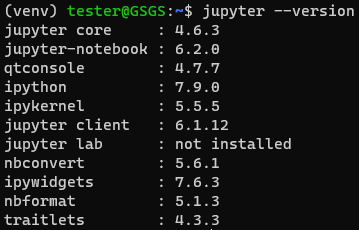
\includegraphics[width=0.4\linewidth]{jupyter_version}
        \caption{Jupyter Notebook 버전 확인}
    \end{center}
\end{figure}

다음 명령어를 입력하여 $\sim$/.jupyter 디렉토리에 접근하자.
\begin{lstlisting}
    $ cd ~/.jupyter
\end{lstlisting}
만약 해당 디렉토리가 존재하지 않는다면, 다음 명령어를 입력하여 해당 디렉토리를 생성한 후 해당 디렉토리에 접근하면 된다.
\begin{lstlisting}
    $ mkdir ~/.jupyter
\end{lstlisting}
이제 다음 명령어를 이용하여 config 파일을 생성하자.
\begin{lstlisting}
    $ jupyter notebook --generate-config
\end{lstlisting}

\begin{figure}[H]
	\begin{center}
        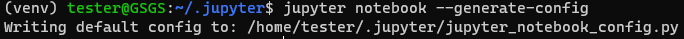
\includegraphics[width=0.8\linewidth]{jupyter_config_generation}
        \caption{Jupyter Notebook config 파일 생성}
    \end{center}
\end{figure}

이제 $\sim$/.jupyter 디렉토리에 jupyter\_notebook\_config.py라는 파일이 생성되었을 것이다. 해당 파w일의 내용을 지우고 다음 내용을 입력하자. 단, username에는 자신의 아이디를, student\_number에는 자신의 학번을 입력한다.
\begin{lstlisting}
    c = get_config()
    c.NotebookApp.allow_origin='*'
    c.NotebookApp.notebook_dir='/home/username'
    c.NotebookApp.ip='115.23.235.135'
    c.NotebookApp.port=student_number
    c.NotebookApp.open_browser=False
\end{lstlisting}
이제 jupyter notebook을 실행시키기 위해 다음 명령어를 입력하자.
\begin{lstlisting}
    $ jupyter notebook --config ~/.jupyter/jupyter_notebook_config.py
\end{lstlisting}
이제 터미널 창에 뜨는 url을 복사하여 접속하면 jupyter notebook을 사용할 수 있다.\\

\begin{figure}[H]
	\begin{center}
        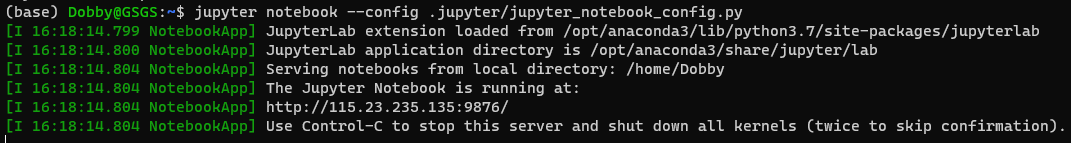
\includegraphics[width=0.6\linewidth]{jupyter_notebook_running}
        \caption{Jupyter Notebook 실행 모습}
    \end{center}
\end{figure}

\begin{figure}[H]
	\begin{center}
        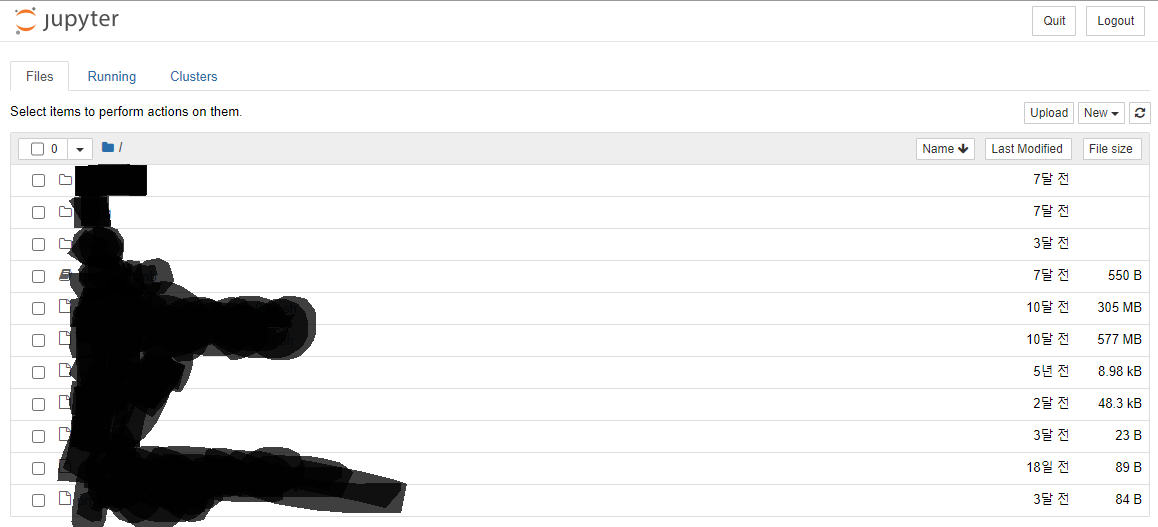
\includegraphics[width=0.8\linewidth]{jupyter_notebook_display}
        \caption{Jupyter Notebook 화면}
    \end{center}
\end{figure}

터미널 창의 세션이 종료되어도 jupyter notebook이 계속 실행되도록 하려면 nohup 명령어를 이용하면 된다.
\begin{lstlisting}
    $ nohup jupyter notebook --config ~/.jupyter/jupyter_notebook_config.py
\end{lstlisting}
